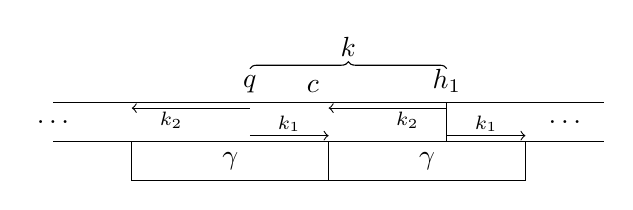
\begin{tikzpicture}[scale=0.5]
    %Boite supérieur et indice
    \draw (3,0)--(17,0);
    \draw (3,1)--(17,1);
    \draw (13,1)--(13,0);
    \node at (3,0.5) {$\dots$};
    \node at (16,0.5) {$\dots$};
    \node[above] at (13,1) {$h_1$};
    \node[above] at (8,1) {$q$};
    \node[above left] at (10,1) {$c$};
    \draw (10,-1) rectangle (15,0) node[pos=.5] {$\gamma$};
    \draw (5,-1) rectangle (10,0) node[pos=.5] {$\gamma$};
    \draw[decoration={brace,raise=5pt},decorate]
    (8,1.5) -- node[above=6pt] {$k$} (13,1.5);
    %Flèche pour $k_i$
    \draw[->] (13,0.85)--(10,0.85);
    \node[below] at (12,1) {\scriptsize $k_2$};
    \draw[->] (8,0.85)--(5,0.85);
    \node[below] at (6,1) {\scriptsize $k_2$};
    \draw[->] (13,0.15)--(15,0.15);
    \node[above] at (9,0) {\scriptsize $k_1$};
    \draw[->] (8,0.15)--(10,0.15);
    \node[above] at (14,0) {\scriptsize $k_1$};
\end{tikzpicture}